\documentclass[a4paper]{book}
\usepackage{a4wide}
\usepackage{makeidx}
\usepackage{fancyhdr}
\usepackage{graphicx}
\usepackage{multicol}
\usepackage{float}
\usepackage{textcomp}
\usepackage{alltt}
\usepackage[utf8]{inputenc}
\usepackage{doxygen}
\makeindex
\setcounter{tocdepth}{3}
\renewcommand{\footrulewidth}{0.4pt}
\begin{document}
\begin{titlepage}
\vspace*{7cm}
\begin{center}
{\Large OpenGLot \\[1ex]\large 0.1 }\\
\vspace*{1cm}
{\large Generated by Doxygen 1.5.8}\\
\vspace*{0.5cm}
{\small Fri Nov 20 18:08:57 2009}\\
\end{center}
\end{titlepage}
\clearemptydoublepage
\pagenumbering{roman}
\tableofcontents
\clearemptydoublepage
\pagenumbering{arabic}
\chapter{Namespace Index}
\section{Namespace List}
Here is a list of all namespaces with brief descriptions:\begin{CompactList}
\item\contentsline{section}{{\bf glot} }{\pageref{namespaceglot}}{}
\end{CompactList}

\chapter{Class Index}
\section{Class Hierarchy}
This inheritance list is sorted roughly, but not completely, alphabetically:\begin{CompactList}
\item \contentsline{section}{glot::color}{\pageref{classglot_1_1color}}{}
\item \contentsline{section}{glot::grapher}{\pageref{classglot_1_1grapher}}{}
\item \contentsline{section}{point}{\pageref{classpoint}}{}
\item \contentsline{section}{glot::primitive}{\pageref{classglot_1_1primitive}}{}
\item \contentsline{section}{ray}{\pageref{classray}}{}
\item \contentsline{section}{rgb}{\pageref{classrgb}}{}
\item \contentsline{section}{screen}{\pageref{structscreen}}{}
\item \contentsline{section}{glot::shader\_\-primitive}{\pageref{classglot_1_1shader__primitive}}{}
\begin{CompactList}
\item \contentsline{section}{glot::surface}{\pageref{classglot_1_1surface}}{}
\end{CompactList}
\item \contentsline{section}{glot::texture}{\pageref{classglot_1_1texture}}{}
\item \contentsline{section}{triangle}{\pageref{classtriangle}}{}
\end{CompactList}

\chapter{Class Index}
\section{Class List}
Here are the classes, structs, unions and interfaces with brief descriptions:\begin{CompactList}
\item\contentsline{section}{{\bf glot::color} }{\pageref{classglot_1_1color}}{}
\item\contentsline{section}{{\bf glot::grapher} }{\pageref{classglot_1_1grapher}}{}
\item\contentsline{section}{{\bf point} }{\pageref{classpoint}}{}
\item\contentsline{section}{{\bf glot::primitive} }{\pageref{classglot_1_1primitive}}{}
\item\contentsline{section}{{\bf ray} }{\pageref{classray}}{}
\item\contentsline{section}{{\bf rgb} }{\pageref{classrgb}}{}
\item\contentsline{section}{{\bf screen} }{\pageref{structscreen}}{}
\item\contentsline{section}{{\bf glot::shader\_\-primitive} }{\pageref{classglot_1_1shader__primitive}}{}
\item\contentsline{section}{{\bf glot::surface} }{\pageref{classglot_1_1surface}}{}
\item\contentsline{section}{{\bf glot::texture} }{\pageref{classglot_1_1texture}}{}
\item\contentsline{section}{{\bf triangle} }{\pageref{classtriangle}}{}
\end{CompactList}

\chapter{File Index}
\section{File List}
Here is a list of all files with brief descriptions:\begin{CompactList}
\item\contentsline{section}{{\bf color.h} }{\pageref{color_8h}}{}
\item\contentsline{section}{{\bf grapher.h} }{\pageref{grapher_8h}}{}
\item\contentsline{section}{{\bf point.h} }{\pageref{point_8h}}{}
\item\contentsline{section}{{\bf primitive.h} }{\pageref{primitive_8h}}{}
\item\contentsline{section}{{\bf ray.h} }{\pageref{ray_8h}}{}
\item\contentsline{section}{{\bf rgb.h} }{\pageref{rgb_8h}}{}
\item\contentsline{section}{{\bf screen.h} }{\pageref{screen_8h}}{}
\item\contentsline{section}{{\bf shader\_\-primitive.h} }{\pageref{shader__primitive_8h}}{}
\item\contentsline{section}{{\bf surface.h} }{\pageref{surface_8h}}{}
\item\contentsline{section}{{\bf texture.h} }{\pageref{texture_8h}}{}
\item\contentsline{section}{{\bf triangle.h} }{\pageref{triangle_8h}}{}
\end{CompactList}

\chapter{Namespace Documentation}
\section{glot Namespace Reference}
\label{namespaceglot}\index{glot@{glot}}
\subsection*{Classes}
\begin{CompactItemize}
\item 
class {\bf color}
\item 
class {\bf grapher}
\item 
class {\bf primitive}
\item 
class {\bf shader\_\-primitive}
\item 
class {\bf surface}
\item 
class {\bf texture}
\end{CompactItemize}
\subsection*{Enumerations}
\begin{CompactItemize}
\item 
enum {\bf display\_\-opt} \{ \par
{\bf AXES\_\-OFF} =  0, 
{\bf GRID\_\-OFF} =  0, 
{\bf X\_\-LIN} =  0, 
{\bf Y\_\-LIN} =  0, 
\par
{\bf AXES\_\-ON} =  1, 
{\bf GRID\_\-ON} =  2, 
{\bf X\_\-LOG} =  4, 
{\bf Y\_\-LOG} =  8
 \}
\begin{CompactList}\small\item\em Enumeration for display options. \item\end{CompactList}\item 
enum {\bf keyboard\_\-opt} \{ \par
{\bf ZOOM\_\-KEYS\_\-OFF} =  0, 
{\bf AXES\_\-KEYS\_\-OFF} =  0, 
{\bf GRID\_\-KEYS\_\-OFF} =  0, 
{\bf ZOOM\_\-KEYS\_\-ON} =  1, 
\par
{\bf AXES\_\-KEYS\_\-ON} =  2, 
{\bf GRID\_\-KEYS\_\-ON} =  4
 \}
\begin{CompactList}\small\item\em Enumeration for keyboard action options. \item\end{CompactList}\end{CompactItemize}


\subsection{Enumeration Type Documentation}
\index{glot@{glot}!display\_\-opt@{display\_\-opt}}
\index{display\_\-opt@{display\_\-opt}!glot@{glot}}
\subsubsection[{display\_\-opt}]{\setlength{\rightskip}{0pt plus 5cm}enum {\bf glot::display\_\-opt}}\label{namespaceglot_48397641a9391dad56e97ef6699ca3e8}


Enumeration for display options. 

Bitwise or these to set the display options \begin{Desc}
\item[Enumerator: ]\par
\begin{description}
\index{AXES\_\-OFF@{AXES\_\-OFF}!glot@{glot}}\index{glot@{glot}!AXES\_\-OFF@{AXES\_\-OFF}}\item[{\em 
AXES\_\-OFF\label{namespaceglot_48397641a9391dad56e97ef6699ca3e8cc985c5059e13185b96eebc3357f1975}
}]\index{GRID\_\-OFF@{GRID\_\-OFF}!glot@{glot}}\index{glot@{glot}!GRID\_\-OFF@{GRID\_\-OFF}}\item[{\em 
GRID\_\-OFF\label{namespaceglot_48397641a9391dad56e97ef6699ca3e8f7f1a13e957aed0fed87a1ca07494c1a}
}]\index{X\_\-LIN@{X\_\-LIN}!glot@{glot}}\index{glot@{glot}!X\_\-LIN@{X\_\-LIN}}\item[{\em 
X\_\-LIN\label{namespaceglot_48397641a9391dad56e97ef6699ca3e8fe22cf1f4facde1c4647411dbf93302b}
}]\index{Y\_\-LIN@{Y\_\-LIN}!glot@{glot}}\index{glot@{glot}!Y\_\-LIN@{Y\_\-LIN}}\item[{\em 
Y\_\-LIN\label{namespaceglot_48397641a9391dad56e97ef6699ca3e8bc26e4ec70a3a053cc9537be8def5e72}
}]\index{AXES\_\-ON@{AXES\_\-ON}!glot@{glot}}\index{glot@{glot}!AXES\_\-ON@{AXES\_\-ON}}\item[{\em 
AXES\_\-ON\label{namespaceglot_48397641a9391dad56e97ef6699ca3e857ca9b6d79f02bf0970b09a1e717e457}
}]\index{GRID\_\-ON@{GRID\_\-ON}!glot@{glot}}\index{glot@{glot}!GRID\_\-ON@{GRID\_\-ON}}\item[{\em 
GRID\_\-ON\label{namespaceglot_48397641a9391dad56e97ef6699ca3e8028b91a09052eb213b4abf6283e78461}
}]\index{X\_\-LOG@{X\_\-LOG}!glot@{glot}}\index{glot@{glot}!X\_\-LOG@{X\_\-LOG}}\item[{\em 
X\_\-LOG\label{namespaceglot_48397641a9391dad56e97ef6699ca3e89ab350a7739d4dc57fff188823f098a0}
}]\index{Y\_\-LOG@{Y\_\-LOG}!glot@{glot}}\index{glot@{glot}!Y\_\-LOG@{Y\_\-LOG}}\item[{\em 
Y\_\-LOG\label{namespaceglot_48397641a9391dad56e97ef6699ca3e807f7ef89539f8db9717d4ff6a84e6385}
}]\end{description}
\end{Desc}

\index{glot@{glot}!keyboard\_\-opt@{keyboard\_\-opt}}
\index{keyboard\_\-opt@{keyboard\_\-opt}!glot@{glot}}
\subsubsection[{keyboard\_\-opt}]{\setlength{\rightskip}{0pt plus 5cm}enum {\bf glot::keyboard\_\-opt}}\label{namespaceglot_cfe91431ea4a54852a727f7834e44086}


Enumeration for keyboard action options. 

Bitwise or these to set the keyboard action options \begin{Desc}
\item[Enumerator: ]\par
\begin{description}
\index{ZOOM\_\-KEYS\_\-OFF@{ZOOM\_\-KEYS\_\-OFF}!glot@{glot}}\index{glot@{glot}!ZOOM\_\-KEYS\_\-OFF@{ZOOM\_\-KEYS\_\-OFF}}\item[{\em 
ZOOM\_\-KEYS\_\-OFF\label{namespaceglot_cfe91431ea4a54852a727f7834e4408650c81ad1bf05a21b32c0027e81bc46f4}
}]\index{AXES\_\-KEYS\_\-OFF@{AXES\_\-KEYS\_\-OFF}!glot@{glot}}\index{glot@{glot}!AXES\_\-KEYS\_\-OFF@{AXES\_\-KEYS\_\-OFF}}\item[{\em 
AXES\_\-KEYS\_\-OFF\label{namespaceglot_cfe91431ea4a54852a727f7834e44086b197d9081ff787f6c9e3b6d93cdcbace}
}]\index{GRID\_\-KEYS\_\-OFF@{GRID\_\-KEYS\_\-OFF}!glot@{glot}}\index{glot@{glot}!GRID\_\-KEYS\_\-OFF@{GRID\_\-KEYS\_\-OFF}}\item[{\em 
GRID\_\-KEYS\_\-OFF\label{namespaceglot_cfe91431ea4a54852a727f7834e4408619a13d43980e118a52f5205844003dc9}
}]\index{ZOOM\_\-KEYS\_\-ON@{ZOOM\_\-KEYS\_\-ON}!glot@{glot}}\index{glot@{glot}!ZOOM\_\-KEYS\_\-ON@{ZOOM\_\-KEYS\_\-ON}}\item[{\em 
ZOOM\_\-KEYS\_\-ON\label{namespaceglot_cfe91431ea4a54852a727f7834e44086bc55dffb01fd33ceffe584ca30adcbab}
}]\index{AXES\_\-KEYS\_\-ON@{AXES\_\-KEYS\_\-ON}!glot@{glot}}\index{glot@{glot}!AXES\_\-KEYS\_\-ON@{AXES\_\-KEYS\_\-ON}}\item[{\em 
AXES\_\-KEYS\_\-ON\label{namespaceglot_cfe91431ea4a54852a727f7834e4408648e6d527976c5a8ba1dacea5d047f891}
}]\index{GRID\_\-KEYS\_\-ON@{GRID\_\-KEYS\_\-ON}!glot@{glot}}\index{glot@{glot}!GRID\_\-KEYS\_\-ON@{GRID\_\-KEYS\_\-ON}}\item[{\em 
GRID\_\-KEYS\_\-ON\label{namespaceglot_cfe91431ea4a54852a727f7834e440868c38cb439a3622ed773d4582272ad552}
}]\end{description}
\end{Desc}


\chapter{Class Documentation}
\section{glot::color Class Reference}
\label{classglot_1_1color}\index{glot::color@{glot::color}}
{\tt \#include $<$color.h$>$}

\subsection*{Public Member Functions}
\begin{CompactItemize}
\item 
{\bf color} (double red=0, double green=0, double blue=0, double alpha=1)
\begin{CompactList}\small\item\em Constructor. \item\end{CompactList}\end{CompactItemize}
\subsection*{Public Attributes}
\begin{CompactItemize}
\item 
double {\bf r}
\begin{CompactList}\small\item\em The red component of the \doxyref{color}{p.}{classglot_1_1color}. \item\end{CompactList}\item 
double {\bf g}
\begin{CompactList}\small\item\em The green component of the \doxyref{color}{p.}{classglot_1_1color}. \item\end{CompactList}\item 
double {\bf b}
\begin{CompactList}\small\item\em The blue component of the \doxyref{color}{p.}{classglot_1_1color}. \item\end{CompactList}\item 
double {\bf a}
\begin{CompactList}\small\item\em The transparency of the \doxyref{color}{p.}{classglot_1_1color} (1 = opaque). \item\end{CompactList}\end{CompactItemize}


\subsection{Constructor \& Destructor Documentation}
\index{glot::color@{glot::color}!color@{color}}
\index{color@{color}!glot::color@{glot::color}}
\subsubsection[{color}]{\setlength{\rightskip}{0pt plus 5cm}glot::color::color (double {\em red} = {\tt 0}, \/  double {\em green} = {\tt 0}, \/  double {\em blue} = {\tt 0}, \/  double {\em alpha} = {\tt 1})\hspace{0.3cm}{\tt  [inline]}}\label{classglot_1_1color_aa1bd417bdab7b47076fbde85ccb2ba9}


Constructor. 

\begin{Desc}
\item[Parameters:]
\begin{description}
\item[{\em red}]- red component of \doxyref{color}{p.}{classglot_1_1color} \item[{\em green}]- green component of \doxyref{color}{p.}{classglot_1_1color} \item[{\em blue}]- blue component of \doxyref{color}{p.}{classglot_1_1color} \item[{\em alpha}]- the transparency of the \doxyref{color}{p.}{classglot_1_1color} \end{description}
\end{Desc}


\subsection{Member Data Documentation}
\index{glot::color@{glot::color}!a@{a}}
\index{a@{a}!glot::color@{glot::color}}
\subsubsection[{a}]{\setlength{\rightskip}{0pt plus 5cm}double {\bf glot::color::a}}\label{classglot_1_1color_c47e5ca02bf2a171e22607409740f827}


The transparency of the \doxyref{color}{p.}{classglot_1_1color} (1 = opaque). 

\index{glot::color@{glot::color}!b@{b}}
\index{b@{b}!glot::color@{glot::color}}
\subsubsection[{b}]{\setlength{\rightskip}{0pt plus 5cm}double {\bf glot::color::b}}\label{classglot_1_1color_638f4163ecba1d756c4bde06acc81aa8}


The blue component of the \doxyref{color}{p.}{classglot_1_1color}. 

\index{glot::color@{glot::color}!g@{g}}
\index{g@{g}!glot::color@{glot::color}}
\subsubsection[{g}]{\setlength{\rightskip}{0pt plus 5cm}double {\bf glot::color::g}}\label{classglot_1_1color_c1cfcfb1ee54d040ab03dc7d952b3ab4}


The green component of the \doxyref{color}{p.}{classglot_1_1color}. 

\index{glot::color@{glot::color}!r@{r}}
\index{r@{r}!glot::color@{glot::color}}
\subsubsection[{r}]{\setlength{\rightskip}{0pt plus 5cm}double {\bf glot::color::r}}\label{classglot_1_1color_fce286e75c4e917163ff02e38f6163c8}


The red component of the \doxyref{color}{p.}{classglot_1_1color}. 



The documentation for this class was generated from the following file:\begin{CompactItemize}
\item 
{\bf color.h}\end{CompactItemize}

\section{glot::grapher Class Reference}
\label{classglot_1_1grapher}\index{glot::grapher@{glot::grapher}}
{\tt \#include $<$grapher.h$>$}

\subsection*{Public Types}
\begin{CompactItemize}
\item 
typedef void($\ast$ {\bf keyboard\_\-function} )(unsigned char key, GLint x, GLint y)
\begin{CompactList}\small\item\em Keyboard event handler typedef. \item\end{CompactList}\item 
typedef void($\ast$ {\bf click\_\-function} )(GLint button, GLint x, GLint y)
\begin{CompactList}\small\item\em Click even handler typedef. \item\end{CompactList}\end{CompactItemize}
\subsection*{Static Public Member Functions}
\begin{CompactItemize}
\item 
static int {\bf initialize} (int argc, char $\ast$$\ast$argv, short int options=AXES\_\-ON$|$GRID\_\-ON$|$X\_\-LIN$|$Y\_\-LIN, short int k\_\-options=ZOOM\_\-KEYS\_\-ON$|$AXES\_\-KEYS\_\-ON$|$GRID\_\-KEYS\_\-ON)
\begin{CompactList}\small\item\em Initialize the \doxyref{grapher}{p.}{classglot_1_1grapher}. \item\end{CompactList}\item 
static void {\bf run} ()
\begin{CompactList}\small\item\em Enter the OpenGL main loop after initialization. \item\end{CompactList}\item 
static void {\bf redraw} ()
\begin{CompactList}\small\item\em User-requested redraw. \item\end{CompactList}\item 
static void {\bf add} ({\bf primitive} \&p)
\begin{CompactList}\small\item\em Add a curve to the plot. \item\end{CompactList}\item 
static void {\bf remove} ({\bf primitive} \&p)
\begin{CompactList}\small\item\em Delete a curve from the plot. \item\end{CompactList}\item 
static void {\bf add} ({\bf shader\_\-primitive} \&p)
\item 
static void {\bf remove} (const {\bf shader\_\-primitive} \&p)
\end{CompactItemize}


\subsection{Member Typedef Documentation}
\index{glot::grapher@{glot::grapher}!click\_\-function@{click\_\-function}}
\index{click\_\-function@{click\_\-function}!glot::grapher@{glot::grapher}}
\subsubsection[{click\_\-function}]{\setlength{\rightskip}{0pt plus 5cm}typedef void($\ast$ {\bf glot::grapher::click\_\-function})(GLint button, GLint x, GLint y)}\label{classglot_1_1grapher_c945e6ebe60c3cfeb0b8768c19a4d5c5}


Click even handler typedef. 

\begin{Desc}
\item[Parameters:]
\begin{description}
\item[{\em button}]- GLint button pressed \item[{\em x}]- GLint x coordinate \item[{\em y}]- GLint y coordinate\end{description}
\end{Desc}
See set\_\-click\_\-function(...) for more details \index{glot::grapher@{glot::grapher}!keyboard\_\-function@{keyboard\_\-function}}
\index{keyboard\_\-function@{keyboard\_\-function}!glot::grapher@{glot::grapher}}
\subsubsection[{keyboard\_\-function}]{\setlength{\rightskip}{0pt plus 5cm}typedef void($\ast$ {\bf glot::grapher::keyboard\_\-function})(unsigned char key, GLint x, GLint y)}\label{classglot_1_1grapher_e11b07f266aff004839c7558599ce34d}


Keyboard event handler typedef. 

\begin{Desc}
\item[Parameters:]
\begin{description}
\item[{\em key}]- unsigned char \item[{\em x}]- GLint x coordinate \item[{\em y}]- GLint y coordinate\end{description}
\end{Desc}
A keyboard event handler accepts a key and x, y coordinates 

\subsection{Member Function Documentation}
\index{glot::grapher@{glot::grapher}!add@{add}}
\index{add@{add}!glot::grapher@{glot::grapher}}
\subsubsection[{add}]{\setlength{\rightskip}{0pt plus 5cm}static void glot::grapher::add ({\bf shader\_\-primitive} \& {\em p})\hspace{0.3cm}{\tt  [inline, static]}}\label{classglot_1_1grapher_89ccaac48b37b8a9cb8e1e43432965cd}


\index{glot::grapher@{glot::grapher}!add@{add}}
\index{add@{add}!glot::grapher@{glot::grapher}}
\subsubsection[{add}]{\setlength{\rightskip}{0pt plus 5cm}static void glot::grapher::add ({\bf primitive} \& {\em p})\hspace{0.3cm}{\tt  [static]}}\label{classglot_1_1grapher_3f3e39caee2ec38dc9c21d6d3c9ed564}


Add a curve to the plot. 

\begin{Desc}
\item[Parameters:]
\begin{description}
\item[{\em c}]- The curve you wish to add to the plot\end{description}
\end{Desc}
If you instantiate a curve, you can add it to the plot with this function. NOTE: This does not automatically request a redisplay. The idea here is that you may be adding several curves at once, and so after adding all of your curves, etc., you should then call \doxyref{grapher::redraw()}{p.}{classglot_1_1grapher_3059b797e6369454e302840427cf1056} \index{glot::grapher@{glot::grapher}!initialize@{initialize}}
\index{initialize@{initialize}!glot::grapher@{glot::grapher}}
\subsubsection[{initialize}]{\setlength{\rightskip}{0pt plus 5cm}static int glot::grapher::initialize (int {\em argc}, \/  char $\ast$$\ast$ {\em argv}, \/  short int {\em options} = {\tt AXES\_\-ON$|$GRID\_\-ON$|$X\_\-LIN$|$Y\_\-LIN}, \/  short int {\em k\_\-options} = {\tt ZOOM\_\-KEYS\_\-ON$|$AXES\_\-KEYS\_\-ON$|$GRID\_\-KEYS\_\-ON})\hspace{0.3cm}{\tt  [static]}}\label{classglot_1_1grapher_f5a295a8e0f6e287cded0514977f9463}


Initialize the \doxyref{grapher}{p.}{classglot_1_1grapher}. 

\begin{Desc}
\item[Parameters:]
\begin{description}
\item[{\em argc}]- same as argc used for OpenGL initialization \item[{\em argv}]- same as argv used for OpenGL initialization \item[{\em options}]- startup options \item[{\em k\_\-options}]- the default keyboard actions options\end{description}
\end{Desc}
Use a bitwise or to select startup options: AXES\_\-ON, AXES\_\-OFF GRID\_\-ON, GRID\_\-OFF X\_\-LIN, X\_\-LOG (linear x scale or logarithmic) Y\_\-LIN, Y\_\-LOG (linear y scale or logarithmic) \index{glot::grapher@{glot::grapher}!redraw@{redraw}}
\index{redraw@{redraw}!glot::grapher@{glot::grapher}}
\subsubsection[{redraw}]{\setlength{\rightskip}{0pt plus 5cm}static void glot::grapher::redraw ()\hspace{0.3cm}{\tt  [static]}}\label{classglot_1_1grapher_3059b797e6369454e302840427cf1056}


User-requested redraw. 

If you create an event handler that will make some changes to the graph, you can make those changes and then request a redraw with this function. \index{glot::grapher@{glot::grapher}!remove@{remove}}
\index{remove@{remove}!glot::grapher@{glot::grapher}}
\subsubsection[{remove}]{\setlength{\rightskip}{0pt plus 5cm}static void glot::grapher::remove (const {\bf shader\_\-primitive} \& {\em p})\hspace{0.3cm}{\tt  [inline, static]}}\label{classglot_1_1grapher_1841ead1a8d6241e5c6f35fdde746a37}


\index{glot::grapher@{glot::grapher}!remove@{remove}}
\index{remove@{remove}!glot::grapher@{glot::grapher}}
\subsubsection[{remove}]{\setlength{\rightskip}{0pt plus 5cm}static void glot::grapher::remove ({\bf primitive} \& {\em p})\hspace{0.3cm}{\tt  [static]}}\label{classglot_1_1grapher_2a89eb6c69bc5101896a050edc5f9e4b}


Delete a curve from the plot. 

\begin{Desc}
\item[Parameters:]
\begin{description}
\item[{\em c}]- The curve you wish to delete from the plot\end{description}
\end{Desc}
If you've plotted a curve, but wish to remove it, you can do so with this function. As with add\_\-curve(...), this does not automatically request a redisplay. \index{glot::grapher@{glot::grapher}!run@{run}}
\index{run@{run}!glot::grapher@{glot::grapher}}
\subsubsection[{run}]{\setlength{\rightskip}{0pt plus 5cm}static void glot::grapher::run ()\hspace{0.3cm}{\tt  [static]}}\label{classglot_1_1grapher_0b2131ed9108518ec725887e4ab6d857}


Enter the OpenGL main loop after initialization. 

In general, you will set up your event handlers, main code, etc., and then when you've gotten everything in place, you call \doxyref{grapher::run()}{p.}{classglot_1_1grapher_0b2131ed9108518ec725887e4ab6d857} to start the program's OpenGL portion. 

The documentation for this class was generated from the following file:\begin{CompactItemize}
\item 
{\bf grapher.h}\end{CompactItemize}

\section{point Class Reference}
\label{classpoint}\index{point@{point}}
{\tt \#include $<$point.h$>$}

\subsection*{Public Member Functions}
\begin{CompactItemize}
\item 
{\bf point} ()
\item 
{\bf point} (double myx, double myy, double myz)
\item 
{\bf ray} {\bf operator-} ({\bf point} other)
\end{CompactItemize}
\subsection*{Public Attributes}
\begin{CompactItemize}
\item 
double {\bf x}
\item 
double {\bf y}
\item 
double {\bf z}
\end{CompactItemize}


\subsection{Constructor \& Destructor Documentation}
\index{point@{point}!point@{point}}
\index{point@{point}!point@{point}}
\subsubsection[{point}]{\setlength{\rightskip}{0pt plus 5cm}point::point ()}\label{classpoint_5fe21d4a4539320bf0f5caf1218d31c8}


\index{point@{point}!point@{point}}
\index{point@{point}!point@{point}}
\subsubsection[{point}]{\setlength{\rightskip}{0pt plus 5cm}point::point (double {\em myx}, \/  double {\em myy}, \/  double {\em myz})}\label{classpoint_1c8b090ce06e64ed183682c2d9f68bfe}




\subsection{Member Function Documentation}
\index{point@{point}!operator-@{operator-}}
\index{operator-@{operator-}!point@{point}}
\subsubsection[{operator-}]{\setlength{\rightskip}{0pt plus 5cm}{\bf ray} point::operator- ({\bf point} {\em other})}\label{classpoint_1efc2cc82a2d7d73323d20da6e70de2f}




\subsection{Member Data Documentation}
\index{point@{point}!x@{x}}
\index{x@{x}!point@{point}}
\subsubsection[{x}]{\setlength{\rightskip}{0pt plus 5cm}double {\bf point::x}}\label{classpoint_9c6b34deaf4900ad4193c17935fd384a}


\index{point@{point}!y@{y}}
\index{y@{y}!point@{point}}
\subsubsection[{y}]{\setlength{\rightskip}{0pt plus 5cm}double {\bf point::y}}\label{classpoint_613f8f0d7352731638b0094e1b958b87}


\index{point@{point}!z@{z}}
\index{z@{z}!point@{point}}
\subsubsection[{z}]{\setlength{\rightskip}{0pt plus 5cm}double {\bf point::z}}\label{classpoint_ab1f0c3682401083b5bf252e7001874f}




The documentation for this class was generated from the following file:\begin{CompactItemize}
\item 
{\bf point.h}\end{CompactItemize}

\section{glot::primitive Class Reference}
\label{classglot_1_1primitive}\index{glot::primitive@{glot::primitive}}
{\tt \#include $<$primitive.h$>$}

\subsection*{Public Member Functions}
\begin{CompactItemize}
\item 
{\bf primitive} (const {\bf color} \&col)
\item 
virtual {\bf $\sim$primitive} ()
\item 
virtual void {\bf dl\_\-gen} (const {\bf screen} \&s)=0
\end{CompactItemize}
\subsection*{Public Attributes}
\begin{CompactItemize}
\item 
{\bf color} {\bf c}
\begin{CompactList}\small\item\em The \doxyref{color}{p.}{classglot_1_1color} of the the \doxyref{point}{p.}{classpoint}. \item\end{CompactList}\item 
GLenum {\bf p}
\end{CompactItemize}


\subsection{Constructor \& Destructor Documentation}
\index{glot::primitive@{glot::primitive}!primitive@{primitive}}
\index{primitive@{primitive}!glot::primitive@{glot::primitive}}
\subsubsection[{primitive}]{\setlength{\rightskip}{0pt plus 5cm}glot::primitive::primitive (const {\bf color} \& {\em col})\hspace{0.3cm}{\tt  [inline]}}\label{classglot_1_1primitive_0e1f934674a70902f0221d7319f18186}


\index{glot::primitive@{glot::primitive}!$\sim$primitive@{$\sim$primitive}}
\index{$\sim$primitive@{$\sim$primitive}!glot::primitive@{glot::primitive}}
\subsubsection[{$\sim$primitive}]{\setlength{\rightskip}{0pt plus 5cm}virtual glot::primitive::$\sim$primitive ()\hspace{0.3cm}{\tt  [inline, virtual]}}\label{classglot_1_1primitive_7c5a2b51466cde951ac85b6c86309cca}




\subsection{Member Function Documentation}
\index{glot::primitive@{glot::primitive}!dl\_\-gen@{dl\_\-gen}}
\index{dl\_\-gen@{dl\_\-gen}!glot::primitive@{glot::primitive}}
\subsubsection[{dl\_\-gen}]{\setlength{\rightskip}{0pt plus 5cm}virtual void glot::primitive::dl\_\-gen (const {\bf screen} \& {\em s})\hspace{0.3cm}{\tt  [pure virtual]}}\label{classglot_1_1primitive_2e8c612e7642561ae3536a865c08a436}




\subsection{Member Data Documentation}
\index{glot::primitive@{glot::primitive}!c@{c}}
\index{c@{c}!glot::primitive@{glot::primitive}}
\subsubsection[{c}]{\setlength{\rightskip}{0pt plus 5cm}{\bf color} {\bf glot::primitive::c}}\label{classglot_1_1primitive_ea0f7ab17148686a80fb68230eb09eba}


The \doxyref{color}{p.}{classglot_1_1color} of the the \doxyref{point}{p.}{classpoint}. 

\index{glot::primitive@{glot::primitive}!p@{p}}
\index{p@{p}!glot::primitive@{glot::primitive}}
\subsubsection[{p}]{\setlength{\rightskip}{0pt plus 5cm}GLenum {\bf glot::primitive::p}}\label{classglot_1_1primitive_e0c4cfa6abb55f0a13c6e12fac732f9b}




The documentation for this class was generated from the following file:\begin{CompactItemize}
\item 
{\bf primitive.h}\end{CompactItemize}

\section{ray Class Reference}
\label{classray}\index{ray@{ray}}
{\tt \#include $<$ray.h$>$}

\subsection*{Public Member Functions}
\begin{CompactItemize}
\item 
{\bf ray} ()
\item 
{\bf ray} (double myx, double myy, double myz)
\item 
double {\bf length} ()
\item 
void {\bf normalize} ()
\item 
{\bf ray} {\bf operator+} ({\bf ray} other)
\item 
void {\bf operator+=} ({\bf ray} other)
\item 
double {\bf operator$\ast$} ({\bf ray} other)
\item 
{\bf ray} {\bf operator/} ({\bf ray} other)
\end{CompactItemize}
\subsection*{Public Attributes}
\begin{CompactItemize}
\item 
double {\bf x}
\item 
double {\bf y}
\item 
double {\bf z}
\end{CompactItemize}


\subsection{Constructor \& Destructor Documentation}
\index{ray@{ray}!ray@{ray}}
\index{ray@{ray}!ray@{ray}}
\subsubsection[{ray}]{\setlength{\rightskip}{0pt plus 5cm}ray::ray ()}\label{classray_6a81906c090ceff40ac9a288639f4861}


\index{ray@{ray}!ray@{ray}}
\index{ray@{ray}!ray@{ray}}
\subsubsection[{ray}]{\setlength{\rightskip}{0pt plus 5cm}ray::ray (double {\em myx}, \/  double {\em myy}, \/  double {\em myz})}\label{classray_5a60830c7f35162a682edf393f24626b}




\subsection{Member Function Documentation}
\index{ray@{ray}!length@{length}}
\index{length@{length}!ray@{ray}}
\subsubsection[{length}]{\setlength{\rightskip}{0pt plus 5cm}double ray::length ()}\label{classray_0998b159ca3d5b7196ee3e8cd7dafd97}


\index{ray@{ray}!normalize@{normalize}}
\index{normalize@{normalize}!ray@{ray}}
\subsubsection[{normalize}]{\setlength{\rightskip}{0pt plus 5cm}void ray::normalize ()}\label{classray_f715b58c77ef3e8d75b4058af13bda57}


\index{ray@{ray}!operator$\ast$@{operator$\ast$}}
\index{operator$\ast$@{operator$\ast$}!ray@{ray}}
\subsubsection[{operator$\ast$}]{\setlength{\rightskip}{0pt plus 5cm}double ray::operator$\ast$ ({\bf ray} {\em other})}\label{classray_3a6a56ccec9972dc3914e07b8ee6b15f}


\index{ray@{ray}!operator+@{operator+}}
\index{operator+@{operator+}!ray@{ray}}
\subsubsection[{operator+}]{\setlength{\rightskip}{0pt plus 5cm}{\bf ray} ray::operator+ ({\bf ray} {\em other})}\label{classray_018669471c0e2e0c5e5b0c78a6773535}


\index{ray@{ray}!operator+=@{operator+=}}
\index{operator+=@{operator+=}!ray@{ray}}
\subsubsection[{operator+=}]{\setlength{\rightskip}{0pt plus 5cm}void ray::operator+= ({\bf ray} {\em other})}\label{classray_dee2a59aa24f6bc20eebe68c1daaf909}


\index{ray@{ray}!operator/@{operator/}}
\index{operator/@{operator/}!ray@{ray}}
\subsubsection[{operator/}]{\setlength{\rightskip}{0pt plus 5cm}{\bf ray} ray::operator/ ({\bf ray} {\em other})}\label{classray_ea9732377ed3684c71f699feef534385}




\subsection{Member Data Documentation}
\index{ray@{ray}!x@{x}}
\index{x@{x}!ray@{ray}}
\subsubsection[{x}]{\setlength{\rightskip}{0pt plus 5cm}double {\bf ray::x}}\label{classray_e9f4259fab216f829be488908bf50658}


\index{ray@{ray}!y@{y}}
\index{y@{y}!ray@{ray}}
\subsubsection[{y}]{\setlength{\rightskip}{0pt plus 5cm}double {\bf ray::y}}\label{classray_d3da4a9ebe44c9977c7049f43be38d97}


\index{ray@{ray}!z@{z}}
\index{z@{z}!ray@{ray}}
\subsubsection[{z}]{\setlength{\rightskip}{0pt plus 5cm}double {\bf ray::z}}\label{classray_9b93204e6fe7898faa4b5c763a2175f1}




The documentation for this class was generated from the following file:\begin{CompactItemize}
\item 
{\bf ray.h}\end{CompactItemize}

\section{rgb Class Reference}
\label{classrgb}\index{rgb@{rgb}}
{\tt \#include $<$rgb.h$>$}

\subsection*{Public Attributes}
\begin{CompactItemize}
\item 
unsigned char {\bf r}
\item 
unsigned char {\bf g}
\item 
unsigned char {\bf b}
\end{CompactItemize}


\subsection{Member Data Documentation}
\index{rgb@{rgb}!b@{b}}
\index{b@{b}!rgb@{rgb}}
\subsubsection[{b}]{\setlength{\rightskip}{0pt plus 5cm}unsigned char {\bf rgb::b}}\label{classrgb_e99e63aa161acf8066058b7af8b3e02c}


\index{rgb@{rgb}!g@{g}}
\index{g@{g}!rgb@{rgb}}
\subsubsection[{g}]{\setlength{\rightskip}{0pt plus 5cm}unsigned char {\bf rgb::g}}\label{classrgb_aa90468fc445cd4003cea65a84dea3e8}


\index{rgb@{rgb}!r@{r}}
\index{r@{r}!rgb@{rgb}}
\subsubsection[{r}]{\setlength{\rightskip}{0pt plus 5cm}unsigned char {\bf rgb::r}}\label{classrgb_2e51db126cff93863d52bb429fbc422d}




The documentation for this class was generated from the following file:\begin{CompactItemize}
\item 
{\bf rgb.h}\end{CompactItemize}

\section{screen Struct Reference}
\label{structscreen}\index{screen@{screen}}
{\tt \#include $<$screen.h$>$}

\subsection*{Public Attributes}
\begin{CompactItemize}
\item 
int {\bf height}
\item 
int {\bf width}
\item 
double {\bf minx}
\item 
double {\bf maxx}
\item 
double {\bf miny}
\item 
double {\bf maxy}
\item 
double {\bf time}
\end{CompactItemize}


\subsection{Member Data Documentation}
\index{screen@{screen}!height@{height}}
\index{height@{height}!screen@{screen}}
\subsubsection[{height}]{\setlength{\rightskip}{0pt plus 5cm}int {\bf screen::height}}\label{structscreen_bf92d5370ef230dd4c6f603435341f50}


\index{screen@{screen}!maxx@{maxx}}
\index{maxx@{maxx}!screen@{screen}}
\subsubsection[{maxx}]{\setlength{\rightskip}{0pt plus 5cm}double {\bf screen::maxx}}\label{structscreen_44a54fff987e77df78e735135c49a06c}


\index{screen@{screen}!maxy@{maxy}}
\index{maxy@{maxy}!screen@{screen}}
\subsubsection[{maxy}]{\setlength{\rightskip}{0pt plus 5cm}double {\bf screen::maxy}}\label{structscreen_ed903ce1e7c63258fff721dd7589d664}


\index{screen@{screen}!minx@{minx}}
\index{minx@{minx}!screen@{screen}}
\subsubsection[{minx}]{\setlength{\rightskip}{0pt plus 5cm}double {\bf screen::minx}}\label{structscreen_ce1577a6c8685aa8aabb3008346ee014}


\index{screen@{screen}!miny@{miny}}
\index{miny@{miny}!screen@{screen}}
\subsubsection[{miny}]{\setlength{\rightskip}{0pt plus 5cm}double {\bf screen::miny}}\label{structscreen_e58c495356145ced9399aa6fe2fe36e4}


\index{screen@{screen}!time@{time}}
\index{time@{time}!screen@{screen}}
\subsubsection[{time}]{\setlength{\rightskip}{0pt plus 5cm}double {\bf screen::time}}\label{structscreen_823fed6a66633783f3d828ac2fdf21dd}


\index{screen@{screen}!width@{width}}
\index{width@{width}!screen@{screen}}
\subsubsection[{width}]{\setlength{\rightskip}{0pt plus 5cm}int {\bf screen::width}}\label{structscreen_5a1821f8d8c202dfbf0755d2162fb64b}




The documentation for this struct was generated from the following file:\begin{CompactItemize}
\item 
{\bf screen.h}\end{CompactItemize}

\section{glot::shader\_\-primitive Class Reference}
\label{classglot_1_1shader__primitive}\index{glot::shader\_\-primitive@{glot::shader\_\-primitive}}
{\tt \#include $<$shader\_\-primitive.h$>$}

Inheritance diagram for glot::shader\_\-primitive::\begin{figure}[H]
\begin{center}
\leavevmode
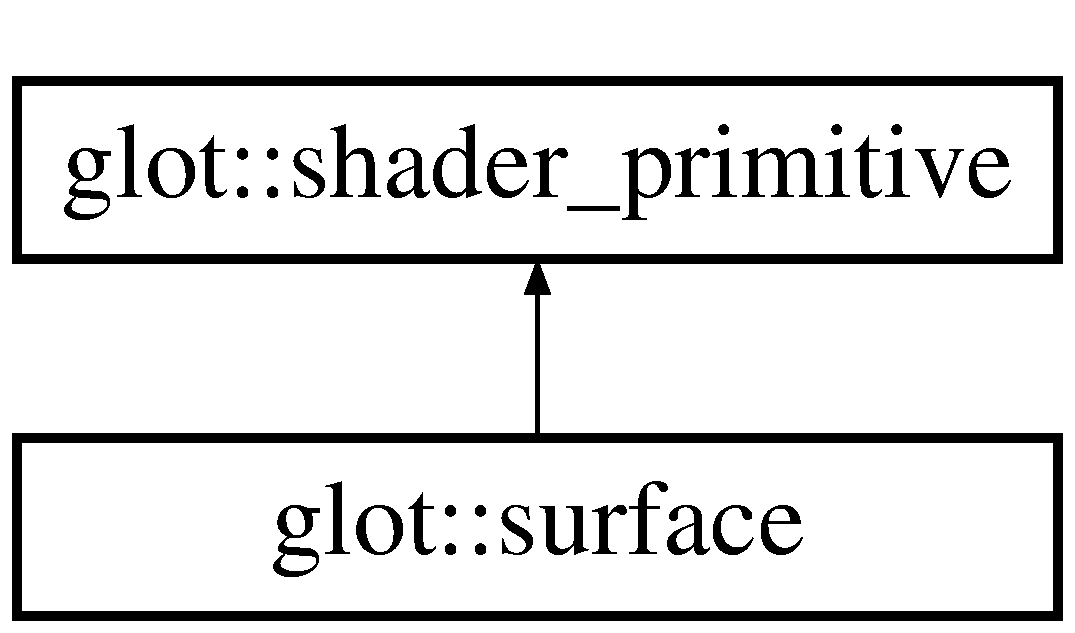
\includegraphics[height=2cm]{classglot_1_1shader__primitive}
\end{center}
\end{figure}
\subsection*{Public Member Functions}
\begin{CompactItemize}
\item 
{\bf shader\_\-primitive} (const {\bf color} \&col)
\item 
virtual {\bf $\sim$shader\_\-primitive} ()
\item 
virtual void {\bf dl\_\-gen} (const {\bf screen} \&s)=0
\item 
void {\bf printProgramInfoLog} (GLuint obj)
\item 
void {\bf printShaderInfoLog} (GLuint obj)
\item 
string {\bf read\_\-file} (const char $\ast$filename)
\end{CompactItemize}
\subsection*{Public Attributes}
\begin{CompactItemize}
\item 
{\bf color} {\bf c}
\begin{CompactList}\small\item\em The \doxyref{color}{p.}{classglot_1_1color} of the the \doxyref{point}{p.}{classpoint}. \item\end{CompactList}\item 
GLenum {\bf p}
\end{CompactItemize}


\subsection{Constructor \& Destructor Documentation}
\index{glot::shader\_\-primitive@{glot::shader\_\-primitive}!shader\_\-primitive@{shader\_\-primitive}}
\index{shader\_\-primitive@{shader\_\-primitive}!glot::shader_primitive@{glot::shader\_\-primitive}}
\subsubsection[{shader\_\-primitive}]{\setlength{\rightskip}{0pt plus 5cm}glot::shader\_\-primitive::shader\_\-primitive (const {\bf color} \& {\em col})\hspace{0.3cm}{\tt  [inline]}}\label{classglot_1_1shader__primitive_1b24678b292e10204f97c7c8c2732a23}


\index{glot::shader\_\-primitive@{glot::shader\_\-primitive}!$\sim$shader\_\-primitive@{$\sim$shader\_\-primitive}}
\index{$\sim$shader\_\-primitive@{$\sim$shader\_\-primitive}!glot::shader_primitive@{glot::shader\_\-primitive}}
\subsubsection[{$\sim$shader\_\-primitive}]{\setlength{\rightskip}{0pt plus 5cm}virtual glot::shader\_\-primitive::$\sim$shader\_\-primitive ()\hspace{0.3cm}{\tt  [inline, virtual]}}\label{classglot_1_1shader__primitive_93bfea81ab50ae43ce5c8812654271f0}




\subsection{Member Function Documentation}
\index{glot::shader\_\-primitive@{glot::shader\_\-primitive}!dl\_\-gen@{dl\_\-gen}}
\index{dl\_\-gen@{dl\_\-gen}!glot::shader_primitive@{glot::shader\_\-primitive}}
\subsubsection[{dl\_\-gen}]{\setlength{\rightskip}{0pt plus 5cm}virtual void glot::shader\_\-primitive::dl\_\-gen (const {\bf screen} \& {\em s})\hspace{0.3cm}{\tt  [pure virtual]}}\label{classglot_1_1shader__primitive_f356a15a35884799e671030ee473dd69}




Implemented in {\bf glot::surface} \doxyref{}{p.}{classglot_1_1surface_ef161d86c3e1402252834e17951d5285}.\index{glot::shader\_\-primitive@{glot::shader\_\-primitive}!printProgramInfoLog@{printProgramInfoLog}}
\index{printProgramInfoLog@{printProgramInfoLog}!glot::shader_primitive@{glot::shader\_\-primitive}}
\subsubsection[{printProgramInfoLog}]{\setlength{\rightskip}{0pt plus 5cm}void glot::shader\_\-primitive::printProgramInfoLog (GLuint {\em obj})}\label{classglot_1_1shader__primitive_1f240d0f05e89e381c35450390128061}


\index{glot::shader\_\-primitive@{glot::shader\_\-primitive}!printShaderInfoLog@{printShaderInfoLog}}
\index{printShaderInfoLog@{printShaderInfoLog}!glot::shader_primitive@{glot::shader\_\-primitive}}
\subsubsection[{printShaderInfoLog}]{\setlength{\rightskip}{0pt plus 5cm}void glot::shader\_\-primitive::printShaderInfoLog (GLuint {\em obj})}\label{classglot_1_1shader__primitive_8ebd19ffbde159147225a276448e35f1}


\index{glot::shader\_\-primitive@{glot::shader\_\-primitive}!read\_\-file@{read\_\-file}}
\index{read\_\-file@{read\_\-file}!glot::shader_primitive@{glot::shader\_\-primitive}}
\subsubsection[{read\_\-file}]{\setlength{\rightskip}{0pt plus 5cm}string glot::shader\_\-primitive::read\_\-file (const char $\ast$ {\em filename})}\label{classglot_1_1shader__primitive_a56ca0b59dd09e40d37670ef74ff1bb9}




\subsection{Member Data Documentation}
\index{glot::shader\_\-primitive@{glot::shader\_\-primitive}!c@{c}}
\index{c@{c}!glot::shader_primitive@{glot::shader\_\-primitive}}
\subsubsection[{c}]{\setlength{\rightskip}{0pt plus 5cm}{\bf color} {\bf glot::shader\_\-primitive::c}}\label{classglot_1_1shader__primitive_19e07023e114aae3bc4a5c48d4a75303}


The \doxyref{color}{p.}{classglot_1_1color} of the the \doxyref{point}{p.}{classpoint}. 



Reimplemented in {\bf glot::surface} \doxyref{}{p.}{classglot_1_1surface_45f4c716c6bfbf9735766d26dce58717}.\index{glot::shader\_\-primitive@{glot::shader\_\-primitive}!p@{p}}
\index{p@{p}!glot::shader_primitive@{glot::shader\_\-primitive}}
\subsubsection[{p}]{\setlength{\rightskip}{0pt plus 5cm}GLenum {\bf glot::shader\_\-primitive::p}}\label{classglot_1_1shader__primitive_c1bbdf9f1a3c6ac2485d022465b990a2}




The documentation for this class was generated from the following file:\begin{CompactItemize}
\item 
{\bf shader\_\-primitive.h}\end{CompactItemize}

\section{glot::surface Class Reference}
\label{classglot_1_1surface}\index{glot::surface@{glot::surface}}
{\tt \#include $<$surface.h$>$}

Inheritance diagram for glot::surface::\begin{figure}[H]
\begin{center}
\leavevmode
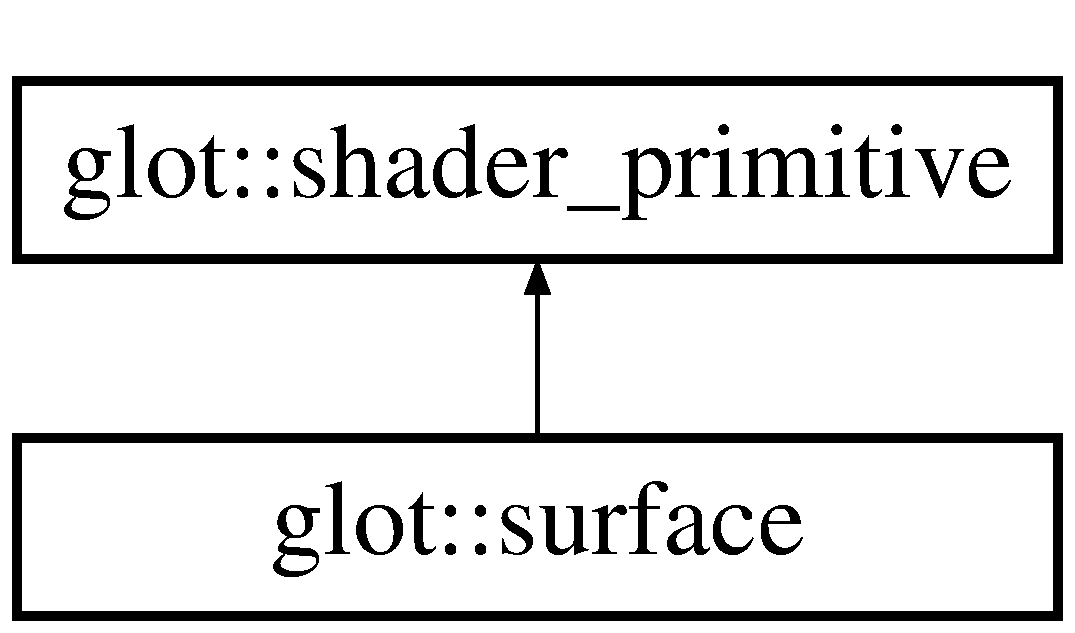
\includegraphics[height=2cm]{classglot_1_1surface}
\end{center}
\end{figure}
\subsection*{Public Member Functions}
\begin{CompactItemize}
\item 
{\bf surface} (const string \&f, const {\bf color} \&col, const string \&filename)
\item 
void {\bf dl\_\-gen} (const {\bf screen} \&s)
\end{CompactItemize}
\subsection*{Public Attributes}
\begin{CompactItemize}
\item 
{\bf color} {\bf c}
\begin{CompactList}\small\item\em The \doxyref{color}{p.}{classglot_1_1color} of the the \doxyref{point}{p.}{classpoint}. \item\end{CompactList}\end{CompactItemize}


\subsection{Constructor \& Destructor Documentation}
\index{glot::surface@{glot::surface}!surface@{surface}}
\index{surface@{surface}!glot::surface@{glot::surface}}
\subsubsection[{surface}]{\setlength{\rightskip}{0pt plus 5cm}glot::surface::surface (const string \& {\em f}, \/  const {\bf color} \& {\em col}, \/  const string \& {\em filename})\hspace{0.3cm}{\tt  [inline]}}\label{classglot_1_1surface_315c81a8238eb8180783fc2989e6b96b}




\subsection{Member Function Documentation}
\index{glot::surface@{glot::surface}!dl\_\-gen@{dl\_\-gen}}
\index{dl\_\-gen@{dl\_\-gen}!glot::surface@{glot::surface}}
\subsubsection[{dl\_\-gen}]{\setlength{\rightskip}{0pt plus 5cm}void glot::surface::dl\_\-gen (const {\bf screen} \& {\em s})\hspace{0.3cm}{\tt  [virtual]}}\label{classglot_1_1surface_ef161d86c3e1402252834e17951d5285}




Implements {\bf glot::shader\_\-primitive} \doxyref{}{p.}{classglot_1_1shader__primitive_f356a15a35884799e671030ee473dd69}.

\subsection{Member Data Documentation}
\index{glot::surface@{glot::surface}!c@{c}}
\index{c@{c}!glot::surface@{glot::surface}}
\subsubsection[{c}]{\setlength{\rightskip}{0pt plus 5cm}{\bf color} {\bf glot::surface::c}}\label{classglot_1_1surface_45f4c716c6bfbf9735766d26dce58717}


The \doxyref{color}{p.}{classglot_1_1color} of the the \doxyref{point}{p.}{classpoint}. 



Reimplemented from {\bf glot::shader\_\-primitive} \doxyref{}{p.}{classglot_1_1shader__primitive_19e07023e114aae3bc4a5c48d4a75303}.

The documentation for this class was generated from the following file:\begin{CompactItemize}
\item 
{\bf surface.h}\end{CompactItemize}

\section{glot::texture Class Reference}
\label{classglot_1_1texture}\index{glot::texture@{glot::texture}}
{\tt \#include $<$texture.h$>$}

\subsection*{Public Member Functions}
\begin{CompactItemize}
\item 
{\bf texture} (const string \&fname)
\item 
{\bf $\sim$texture} ()
\end{CompactItemize}


\subsection{Constructor \& Destructor Documentation}
\index{glot::texture@{glot::texture}!texture@{texture}}
\index{texture@{texture}!glot::texture@{glot::texture}}
\subsubsection[{texture}]{\setlength{\rightskip}{0pt plus 5cm}glot::texture::texture (const string \& {\em fname})\hspace{0.3cm}{\tt  [inline]}}\label{classglot_1_1texture_b4f48efa54bbab9e2838a310efd14a93}


\index{glot::texture@{glot::texture}!$\sim$texture@{$\sim$texture}}
\index{$\sim$texture@{$\sim$texture}!glot::texture@{glot::texture}}
\subsubsection[{$\sim$texture}]{\setlength{\rightskip}{0pt plus 5cm}glot::texture::$\sim$texture ()\hspace{0.3cm}{\tt  [inline]}}\label{classglot_1_1texture_fdb9ffb11d5d7eb19914c9bde92727f8}




The documentation for this class was generated from the following file:\begin{CompactItemize}
\item 
{\bf texture.h}\end{CompactItemize}

\section{triangle Class Reference}
\label{classtriangle}\index{triangle@{triangle}}
{\tt \#include $<$triangle.h$>$}

\subsection*{Public Attributes}
\begin{CompactItemize}
\item 
int {\bf a}
\item 
int {\bf b}
\item 
int {\bf c}
\end{CompactItemize}


\subsection{Member Data Documentation}
\index{triangle@{triangle}!a@{a}}
\index{a@{a}!triangle@{triangle}}
\subsubsection[{a}]{\setlength{\rightskip}{0pt plus 5cm}int {\bf triangle::a}}\label{classtriangle_340b2485aa1ed76572a2980f873cfaa2}


\index{triangle@{triangle}!b@{b}}
\index{b@{b}!triangle@{triangle}}
\subsubsection[{b}]{\setlength{\rightskip}{0pt plus 5cm}int {\bf triangle::b}}\label{classtriangle_8b581b74579c237bb7988d4e4e6bb377}


\index{triangle@{triangle}!c@{c}}
\index{c@{c}!triangle@{triangle}}
\subsubsection[{c}]{\setlength{\rightskip}{0pt plus 5cm}int {\bf triangle::c}}\label{classtriangle_2b3ee36792f25bf2a29b2db2683badce}




The documentation for this class was generated from the following file:\begin{CompactItemize}
\item 
{\bf triangle.h}\end{CompactItemize}

\chapter{File Documentation}
\section{color.h File Reference}
\label{color_8h}\index{color.h@{color.h}}
\subsection*{Classes}
\begin{CompactItemize}
\item 
class {\bf glot::color}
\end{CompactItemize}
\subsection*{Namespaces}
\begin{CompactItemize}
\item 
namespace {\bf glot}
\end{CompactItemize}

\section{grapher.h File Reference}
\label{grapher_8h}\index{grapher.h@{grapher.h}}
{\tt \#include $<$GL/glew.h$>$}\par
{\tt \#include $<$GLUT/glut.h$>$}\par
{\tt \#include $<$list$>$}\par
{\tt \#include $<$map$>$}\par
{\tt \#include \char`\"{}shader\_\-primitive.h\char`\"{}}\par
{\tt \#include \char`\"{}primitive.h\char`\"{}}\par
{\tt \#include \char`\"{}surface.h\char`\"{}}\par
{\tt \#include \char`\"{}screen.h\char`\"{}}\par
{\tt \#include \char`\"{}point.h\char`\"{}}\par
\subsection*{Classes}
\begin{CompactItemize}
\item 
class {\bf glot::grapher}
\end{CompactItemize}
\subsection*{Namespaces}
\begin{CompactItemize}
\item 
namespace {\bf glot}
\end{CompactItemize}
\subsection*{Enumerations}
\begin{CompactItemize}
\item 
enum {\bf glot::display\_\-opt} \{ \par
{\bf glot::AXES\_\-OFF} =  0, 
{\bf glot::GRID\_\-OFF} =  0, 
{\bf glot::X\_\-LIN} =  0, 
{\bf glot::Y\_\-LIN} =  0, 
\par
{\bf glot::AXES\_\-ON} =  1, 
{\bf glot::GRID\_\-ON} =  2, 
{\bf glot::X\_\-LOG} =  4, 
{\bf glot::Y\_\-LOG} =  8
 \}
\begin{CompactList}\small\item\em Enumeration for display options. \item\end{CompactList}\item 
enum {\bf glot::keyboard\_\-opt} \{ \par
{\bf glot::ZOOM\_\-KEYS\_\-OFF} =  0, 
{\bf glot::AXES\_\-KEYS\_\-OFF} =  0, 
{\bf glot::GRID\_\-KEYS\_\-OFF} =  0, 
{\bf glot::ZOOM\_\-KEYS\_\-ON} =  1, 
\par
{\bf glot::AXES\_\-KEYS\_\-ON} =  2, 
{\bf glot::GRID\_\-KEYS\_\-ON} =  4
 \}
\begin{CompactList}\small\item\em Enumeration for keyboard action options. \item\end{CompactList}\end{CompactItemize}

\section{point.h File Reference}
\label{point_8h}\index{point.h@{point.h}}
{\tt \#include \char`\"{}ray.h\char`\"{}}\par
\subsection*{Classes}
\begin{CompactItemize}
\item 
class {\bf point}
\end{CompactItemize}

\section{primitive.h File Reference}
\label{primitive_8h}\index{primitive.h@{primitive.h}}
{\tt \#include \char`\"{}screen.h\char`\"{}}\par
{\tt \#include \char`\"{}color.h\char`\"{}}\par
\subsection*{Classes}
\begin{CompactItemize}
\item 
class {\bf glot::primitive}
\end{CompactItemize}
\subsection*{Namespaces}
\begin{CompactItemize}
\item 
namespace {\bf glot}
\end{CompactItemize}

\section{ray.h File Reference}
\label{ray_8h}\index{ray.h@{ray.h}}
\subsection*{Classes}
\begin{CompactItemize}
\item 
class {\bf ray}
\end{CompactItemize}

\section{rgb.h File Reference}
\label{rgb_8h}\index{rgb.h@{rgb.h}}
\subsection*{Classes}
\begin{CompactItemize}
\item 
class {\bf rgb}
\end{CompactItemize}

\section{screen.h File Reference}
\label{screen_8h}\index{screen.h@{screen.h}}
\subsection*{Classes}
\begin{CompactItemize}
\item 
struct {\bf screen}
\end{CompactItemize}

\section{shader\_\-primitive.h File Reference}
\label{shader__primitive_8h}\index{shader\_\-primitive.h@{shader\_\-primitive.h}}
{\tt \#include $<$fstream$>$}\par
{\tt \#include $<$string$>$}\par
{\tt \#include $<$GL/glew.h$>$}\par
{\tt \#include \char`\"{}primitive.h\char`\"{}}\par
{\tt \#include \char`\"{}screen.h\char`\"{}}\par
{\tt \#include \char`\"{}color.h\char`\"{}}\par
\subsection*{Classes}
\begin{CompactItemize}
\item 
class {\bf glot::shader\_\-primitive}
\end{CompactItemize}
\subsection*{Namespaces}
\begin{CompactItemize}
\item 
namespace {\bf glot}
\end{CompactItemize}

\section{surface.h File Reference}
\label{surface_8h}\index{surface.h@{surface.h}}
{\tt \#include $<$GL/glew.h$>$}\par
{\tt \#include $<$string$>$}\par
{\tt \#include \char`\"{}shader\_\-primitive.h\char`\"{}}\par
{\tt \#include \char`\"{}texture.h\char`\"{}}\par
{\tt \#include \char`\"{}color.h\char`\"{}}\par
\subsection*{Classes}
\begin{CompactItemize}
\item 
class {\bf glot::surface}
\end{CompactItemize}
\subsection*{Namespaces}
\begin{CompactItemize}
\item 
namespace {\bf glot}
\end{CompactItemize}

\section{texture.h File Reference}
\label{texture_8h}\index{texture.h@{texture.h}}
{\tt \#include $<$iostream$>$}\par
{\tt \#include $<$string$>$}\par
\subsection*{Classes}
\begin{CompactItemize}
\item 
class {\bf glot::texture}
\end{CompactItemize}
\subsection*{Namespaces}
\begin{CompactItemize}
\item 
namespace {\bf glot}
\end{CompactItemize}

\section{triangle.h File Reference}
\label{triangle_8h}\index{triangle.h@{triangle.h}}
\subsection*{Classes}
\begin{CompactItemize}
\item 
class {\bf triangle}
\end{CompactItemize}

\printindex
\end{document}
